%----------------------------------------------------------------------------------------
%	PACKAGES AND OTHER DOCUMENT CONFIGURATIONS
%----------------------------------------------------------------------------------------

\documentclass{article} % paper and 12pt font size

\newcommand\tab[1][1cm]{\hspace*{#1}}
\def\changemargin#1#2{\list{}{\rightmargin#2\leftmargin#1}\item[]}
\let\endchangemargin=\endlist 

\usepackage{amsmath,amsfonts,amsthm} % Math packages
\usepackage{fancyhdr}
\usepackage[catalan]{babel}
\usepackage[utf8]{inputenc}
\usepackage[T1]{fontenc}
\usepackage{xcolor}
\usepackage{textcomp}
\usepackage{graphicx}
\usepackage{float}
\usepackage{listings}
\usepackage{enumitem}
\usepackage{textgreek}
\usepackage{multirow,tabularx}
\graphicspath{ {img/} }
\setlength\parindent{0pt} % Removes all indentation from paragraphs - comment this line for an assignment with lots of text

\pagestyle{fancy}
\fancyhf{}
\lhead{Pràctica - Aprenentatge computacional}
\rhead{Jordi Alvaro Arqués}
\cfoot{\thepage}

\begin{document}


\section{Exercici 1. Random kNN (RkNN) (20\%)}
El kNN és un algorisme basat en exemples molt utilitzat. Moltes vegades no s'utilitza en la seva forma bàsica, existeixen multiples variants. Una proposta de modificació recent
consisteix en utilitzar varis kNN aplicats en subconjunts aleatoris d’atributs, semblant a la idea del classificador Random Forest (RF) però en comptes d’utilitzar arbres de decisió utilitzar varis classificadors kNN. El resultat del classificador RkNN en una dada de test serà el vot majoritari de tots els kNN utilitzats. La implementació RkNN també pot servir per seleccionar els atributs més significatius (vindran del subconjunt de kNN que tinguin millor
precisió de classificació). \\

Cerqueu informació sobre aquesta modificació i descriviu-la en detall, posant l’ènfasi en com es podria implementar tant la classificació utiltizant RkNN, com es pot implementar la selecció de característiques (ajuda: podeu cercar el següent article “Li S, Harner EJ, Adjeroh DA. Random KNN feature selection - a fast and stable alternative to Random Forests. BMC Bioinformatics. 2011;12:450. doi:10.1186/1471-2105-12-450”). \\

{\color{blue}
	\section*{RkNN:}
	\subsection*{Fase de selecció de característiques:}
	S'escolliran $m$ característiques aleatòriament per a cadascun dels $r$ classificadors kNN que es crearan.

	\subsection*{Fase de creació del classificador:}
	Es creen $r$ classificadors kNN cadascun amb les seves $m$ característiques escollides aleatòriament a la fase anterior. \\

	La predicció s'obtindrà a partir de tots els resultats parcials  dels kNN (cada kNN del conjunt té un sol vot), escollint com a valor final de l'opció més votada.

	\section*{RkNN-FS:}
	\subsection*{Fase de selecció de característiques:}
	El RkNN-FS és un procés de selecció de les característiques més rellevants i que més informació aporten d'un conjunt de dades per a la seva classificació. És un mètode pensat per a resoldre problemes del tipus "small $n$, large $p$". Amb aquest mètode es pot aconseguir reduir molt la dimensionalitat de les dades inicials. \\

	Abans d'explicar els passos d'aquesta fase, cal comentar que a l'article de l'enunciat de l'exercici proposa dos formes de particionat de les dades d'entrada en dos conjunts que serviran de training i testing respectivament. Els dos mètodes de particionat que planteja són els següents:
	\begin{enumerate}
		\item Particionat dinàmic: Per a cada kNN, les dades es divideixen aleatòriament. Una meitat és usada com a dades d'entrenament i l'altra meitat com a dades de test. Per tant, cada kNN tindrà el seu conjunt particular de dades de training i testing.
		\item Les dades es divideixen aleatòriament una única vegada per a tots els kNNs. El mateix conjunt de training i testing és usat per a tots els classificadors.
	\end{enumerate}
	Per a la diversitat dels classificadors de tipus kNN, es recomana el \textbf{particionat dinàmic}. \\

	Dit això, a continuació es mostren els passos per a l'execució de \textbf{RkNN-FS}:

	\begin{enumerate}
		\item{
			El següent procés es repeteix $r$ vegades (així, s'obtindran $r$ classificadors kNN). A l'article científic que s'ens ha proporcionat es comenta que l'$accuracy$ d'aquest algoritme millora a mesura que s'incrementa el valor de $r$, però que per a valors de $r > 1000$ ja no es nota cap millora:

			\begin{enumerate}
				\item Es divideix les dades d'entrada aleatòriament en dos conjunts que serviran de training i testing respectivament. S'utilitza el particionat dinàmic explicat anteriorment.
				\item A partir del conjunt de training, es crea un classificador kNN amb \textit{m} característiques escollides aleatòriament. Normalment, es recomana $m = \sqrt{p}$ (on $p$ és el nombre de característiques de les dades originals) per tal de maximitzar les diferències entre els subconjunts.
				\item Un cop creat el classificador kNN, s'utilitza les dades de testing per a obtenir les prediccions (utilitzant, només, les $m$ característiques seleccionades).
				\item Es compara els valors de les prediccions amb els reals (ground truth) i es calcula l'\textit{accuracy} d'aquest classificador.
			\end{enumerate}
		}
		
		\item{
			A continuació, es calcula la funció de \textit{support} per a cada característica ($p$ en total). Això, consisteix en, per a cada característica, fer la mitjana dels valors de l'\textit{accuracy} dels kNN que l'hagin utilitzat. És a dir:\\
			\[support_{f_i} = \frac{1}{\lvert C_{f_i}\lvert} \sum_{kNN\ \in\ C_{f_i}}^{} acc_{kNN} \quad \lvert \quad \forall i \in \{1, 2, ..., p\}\] \\
			on $C_{f_i}$ és la llista dels classificadors kNN que han usat la característica $f_i$. \\
			Per exemple, suposem que tenim un total de $r = 10$ classificadors i $p = 100$ característiques. I, si una característica $f_1$ només s'ha utilitzat en els classificadors 1, 4 i 6; per saber el valor de la seva funció $support$ s'haurà de calcular: \[support_{f_1} = \frac{acc_{kNN_1} + acc_{kNN_4} + acc_{kNN_6}}{3}\]
		}
		\item {
			Un cop ja tenim calculada la funció de $support$, la selecció de les característiques es pot encarar de dues maneres:
			\begin{enumerate}
				\item Selecció directa. S'escullen directament un nombre determinat de característiques que han obtingut un valor més elevat a la funció de $support$. Tot i la simplicitat d'aquesta estratègia, pot ser una mica massa agressiva i arriscada per a dades amb una alta dimensionalitat.
				\item{
					Utilitzar un enfoc més conservador i prudent. Consisteix en fer vàries iteracions dels passos anteriors (1 i 2) aplicant el procés de selecció directa recursivament. \\
					Per tal d'arribar a un equilibri entre la velocitat i el rendiment de la classificació, es divideix aquest procés d'iteració en dos etapes:
					\begin{enumerate}
						\item {
							Reducció geomètrica de les característiques. Aquesta primera etapa és ràpida, i les variables s'eliminen a un ràtio fixat (per defecte, de $q = 1/2$) en cada iteració. \\
							En aquesta fase de reducció geomètrica es fa el següent:
							\begin{enumerate}
								\item {
									Es calcula el nombre d'iteracions d'aquesta fase:
									\[n_g = \left \lfloor{\frac{\ln(p_{min}/p_{g\ 0})}{\ln(1-q)}}\right \rfloor \]
									on $p_{g\ 0}$ és el nombre de característiques de les dades originals i que s'utilitzaran a la iteració 0 ($p_{g\ 0} = p$), $q$ és el ratio d'eliminació de característiques a cada iteració i $p_{min}$ és el mínim nombre de característiques que l'última iteració utilitzarà. Així, es garanteix que l'última iteració ($n_g - 1$) contindrà com a mínim $p_{min}$ característiques. \\
								}
								\item {
									S'executen les $n_g$ iteracions. Per a cada iteració, es repeteixen els passos 1 i 2 anteriors. Així, es calcula la funció $support$ i el valor mitjà de l'$accuracy$ de tots els kNN. Tal i com ja s'ha comentat, la funció $support$ s'utilitza per a determinar quines característiques s'han de seleccionar per a la següent iteració. També, es té en compte el ratio $q$ seleccionat per tal de saber el nombre de característiques de les següents iteracions:
									\[p_{g\ i+1} = p_{g\ i} \cdot (1 - q) \]
								}
								\item Llavors, al final de totes les iteracions, s'obté una mesura que dóna el valor mitjà de l'$accuracy$ dels kNN per a cada ronda.
								\item A partir d'aquesta mesura, es busca la iteració en la que s'ha obtingut el valor mitjà màxim de l'$accuracy$ dels kNN i se selecciona la iteració prèvia (anomenada \textit{pre-max}).
							\end{enumerate}
						}
						\item {
							Reducció lineal de les característiques. En aquesta etapa, un nombre fixat de característiques (una per defecte) es descarten a cada iteració. \\
							En aquesta fase de reducció geomètrica es fa el següent:
							\begin{enumerate}
								\item{
									Es pren com a punt de partida la iteració \textit{pre-max} obtinguda a la fase anterior (amb les característiques usades en aquella ronda) i s'inicia aquesta fase de reducció lineal. \\
									El nombre d'iteracions d'aquesta fase ve fixat per:
									\[n_l = \left \lfloor{(p_{l\ 0}-p_{min})/d}\right \rfloor \]
									on $d$ és el nombre de característiques a ser eliminades en cada iteració, $p_{l\ 0}$ és el nombre de característiques usades a la iteració 0 (que correspon amb el nombre de característiques usades a la ronda \textit{pre-max} de la fase de reducció geomètrica, $p_{l\ 0} = p_{g\ pre-max}$) i $p_{min}$ és el mínim nombre de característiques que l'última iteració utilitzarà. Així, es garanteix que l'última iteració contindrà com a mínim $p_{min}$ característiques. \\
								}
								\item {
									S'executen les $n_l$ iteracions. Per a cada iteració, es repeteixen els passos 1 i 2 anteriors. Així, es calcula la funció $support$ i el valor mitjà de l'$accuracy$ de tots els kNN. El procediment és el mateix que a la fase de reducció geomètrica, excepte que el nombre de característiques seleccionades en cada iteració no ve fixat per un ràtio, sinó pel valor $d$:
									\[p_{l\ i+1} = p_{l\ i} - d \]
								}
								\item Al final de totes les iteracions, s'obté una mesura que dóna el valor mitjà de l'$accuracy$ dels kNN per a cada ronda.
								\item A partir d'aquesta mesura, es busca la iteració en la que s'ha obtingut el valor mitjà màxim de l'$accuracy$ dels kNN i, en aquest cas, se selecciona aquesta iteració.
								\item Les característiques utilitzades a la iteració seleccionada en el pas anterior seran el conjunt de \textbf{característiques finals} que el mètode \textbf{RkNN-FS} haurà seleccionat.
							\end{enumerate}
						}
					\end{enumerate}
				}
			\end{enumerate}
		}
	\end{enumerate}

	\subsection*{Fase de creació del classificador:}

	Un cop s'han seleccionat les característiques més importants i que aporten més informació alhora de poder classificar correctament les dades d'entrada, es crea un classificador, del tipus que es vulgui (una opció és el kNN), on només es tindran en compte aquestes característiques.
}

\section{Exercici 2. kNN (20\%)}
Dividiu les dades amb conjunts de train i test i utilitzeu l’algoritme kNN original per classificar les dades de test. Doneu els resultats mitjançant precisió i matriu de confusió. Podeu utilitzar la implementació kNN de les PACs anteriors en Python (i scikit-learn, vegeu KneighborsClassifier). \\

{\color{blue}
	Les dades s'han dividit aleatòriament en dos grups d'igual grandària, un per a l'entrenament i l'altre per al testing dels algoritmes. S'ha executat els següents algoritmes: 1NN, 3NN i RkNN (sense selecció de característiques). \\

	L'algoritme RkNN s'ha executat amb els següents paràmetres:
	\begin{enumerate}
		\item $k = 1$ i $k = 3$. S'ha volgut comparar l'algoritme kNN amb els dos valors normalment més usats.
		\item $r = 1000$. S'ha escollit aquest valor, ja que, tal i com es comenta a l'article científic que se'ns ha facilitat, el rendiment de l'algoritme RkNN-FS (en termes d'$accuracy$) millora incrementant $r$, però per a valors de $r > 1000$ ja no es nota cap millora. Llavors, he cregut interessant aplicar el mateix valor per al RkNN.
		\item $m = \left \lceil{\sqrt{p}}\right \rceil$, que en el nostre cas és $m = \left \lceil{\sqrt{13}}\right \rceil = 4$. S'ha escollit aquest valor ja que a l'article, també es comenta ajuda a maximitzar les diferències entre els subconjunts de les característiques escollides.
	\end{enumerate}

	Els resultats d'una execució són els següents:

	\begin{changemargin}{-1.2cm}{0.5cm}
	{\fontfamily{pcr}\selectfont\small
	\begin{tabular}{l | r r r r r}
		& 1NN & 3NN & RkNN (k=1) & RkNN (k=3) \\ \hline
		Train times 				& 0.3237 ms & 0.3061 ms & 296.8227 ms 	& 301.5542 ms\\
		Predict times 				& 0.5631 ms & 0.5829 ms & 456.8302 ms 	& 495.7835 ms\\
		Accuracy 					& 96.63\% 	& 94.38\%	& 98.88\% 		& 96.63\%	 \\
		Classificacions correctes 	& 86 		& 84		& 88			& 86		 \\
		Classificacions incorrectes & 3 		& 5 		& 1				& 3			 \\
	\end{tabular}
	}
	\end{changemargin}

	i les seves matrius de confusió:
	\begin{figure}[H]
		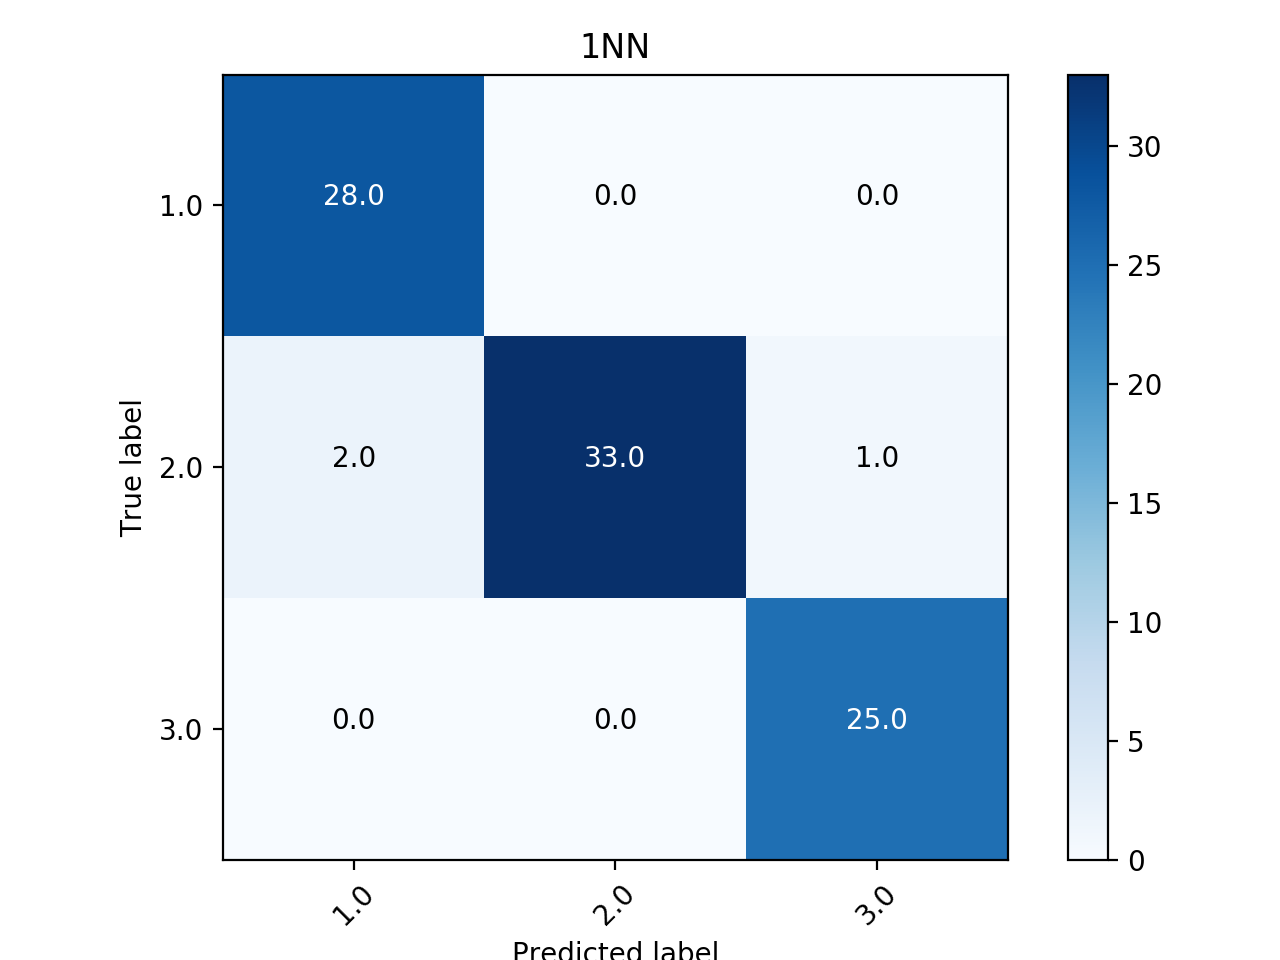
\includegraphics[width=10cm]{1nn}
		\centering
		\color{blue}
		\caption{Matriu de confusió (algoritme 1NN) creada a partir d'una execució sobre les dades d'entrada.}\label{visina8}
	\end{figure}

	\begin{figure}[H]
		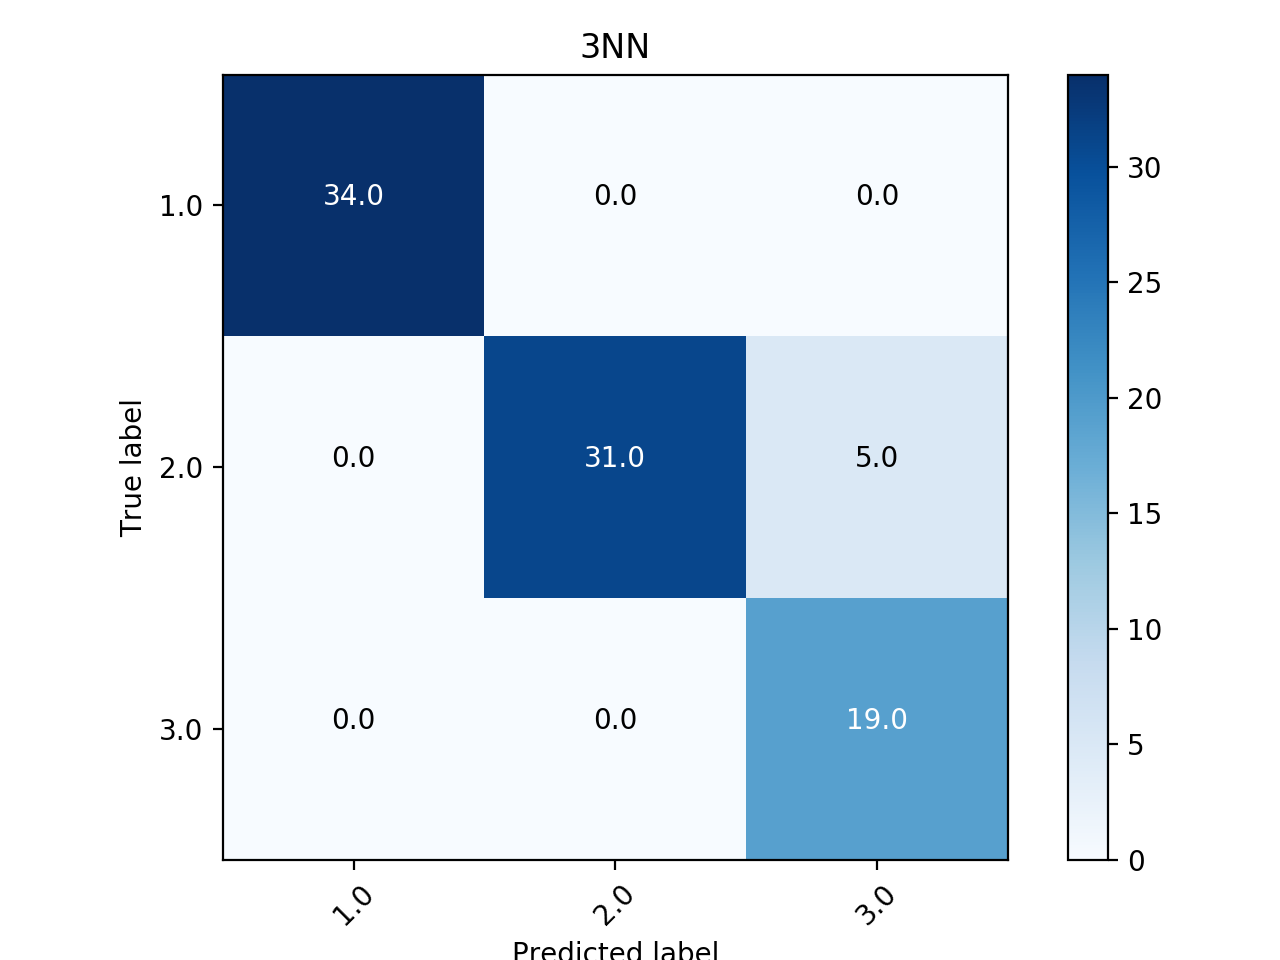
\includegraphics[width=10cm]{3nn}
		\centering
		\color{blue}
		\caption{Matriu de confusió (algoritme 3NN) creada a partir d'una execució sobre les dades d'entrada.}\label{visina8}
	\end{figure}

	\begin{figure}[H]
		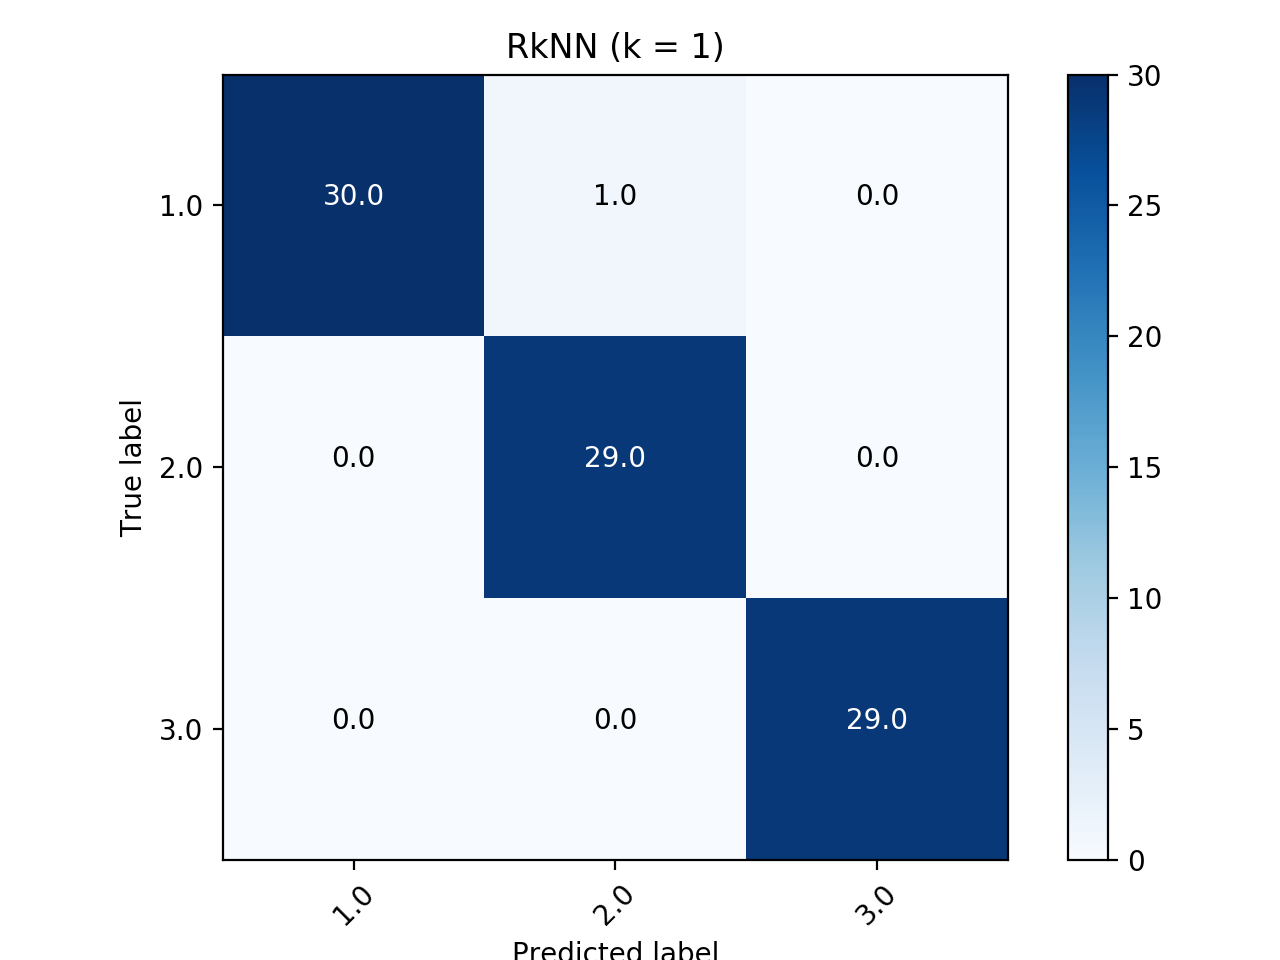
\includegraphics[width=10cm]{r1nn}
		\centering
		\color{blue}
		\caption{Matriu de confusió (algoritme RkNN amb k=1) creada a partir d'una execució sobre les dades d'entrada.}\label{visina8}
	\end{figure}

	\begin{figure}[H]
		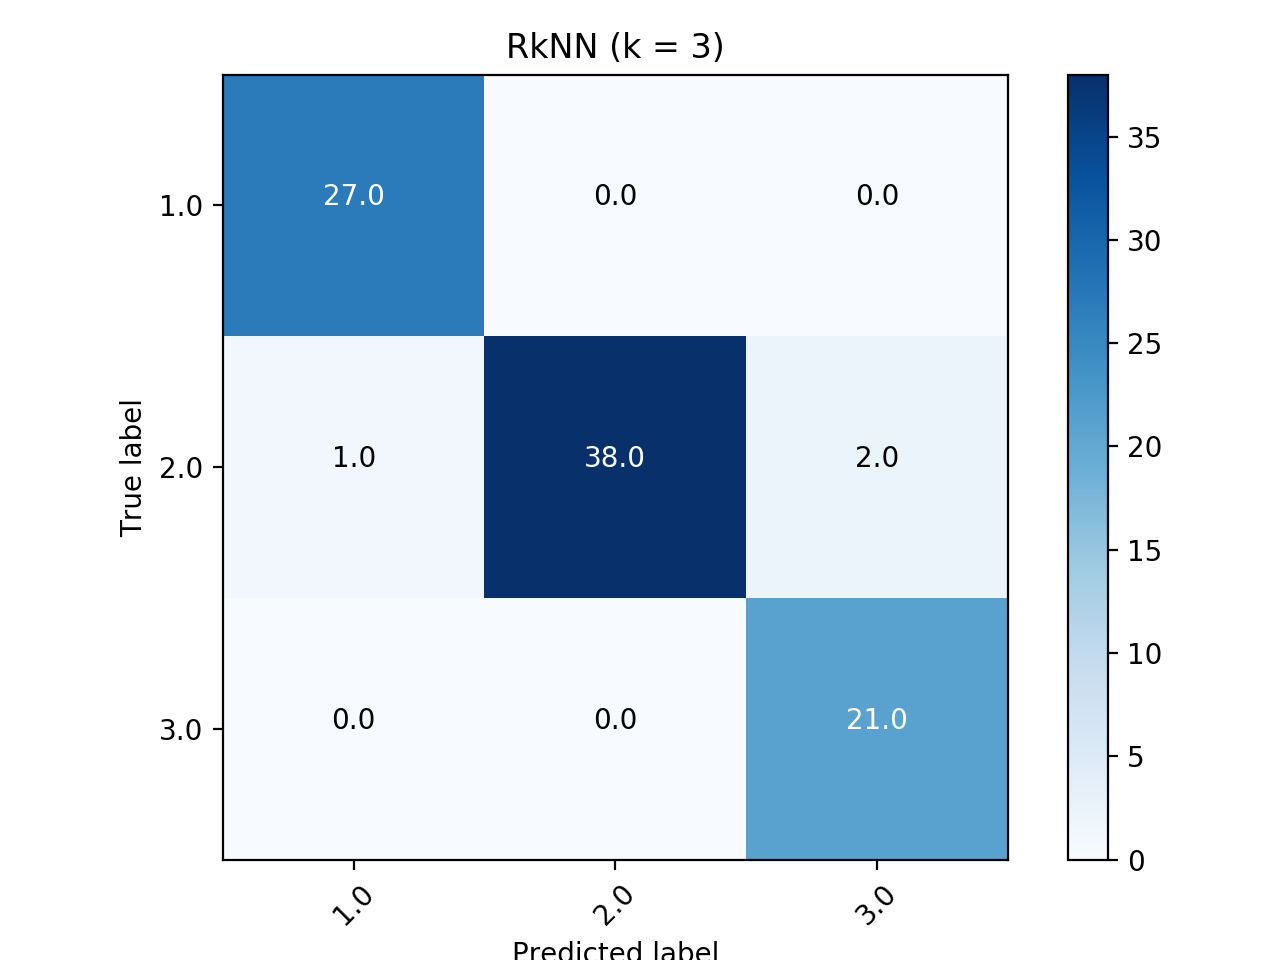
\includegraphics[width=10cm]{r3nn}
		\centering
		\color{blue}
		\caption{Matriu de confusió (algoritme RkNN amb k=3) creada a partir d'una execució sobre les dades d'entrada.}\label{visina8}
	\end{figure}

	Aquests resultats, tal i com s'ha comentat, són el resultat d'una sola execució. S'ha executat múltiples vegades aquests algoritmes de forma manual i s'ha pogut observar que els valors de les $accuracies$ oscil·laven entre el 90\% i el 100\% en el millor dels casos. Així que no s'hi aprecien grans diferències. \\

	Si es volgués estudiar més a fons aquests algoritmes i obtenir uns resultats estadístics i més significatius (la qual cosa queda fora de l'abast d'aquest exercici), s'hauria d'iterar el procés un cert nombre de vegades per a tenir una mostra suficientment significativa i obtenir els valors mitjans i la desviació estàndar. \\

	El que sí que es pot apreciar, és que, aproximadament, l'algoritme RkNN en comparació als kNN (tant a la fase d'entrenament com a la de predicció) és unes 850 vegades més lent. Això, té sentit, ja que hem utilitzat un $r = 1000$, és a dir, el RkNN està realitzant 1000 classificadors kNN internament. No és unes 1000 vegades més lent ja que els programes, quan porten una estona funcionant augmenten la seva eficiència i rendiment.
}

\section{Exercici 3. Implementació del RkNN (60\%)}
Implementeu el kNN amb la modificació de l'exercici 1. Apliqueu la implementació per classificar els mateixos casos de test obtinguts en l’exercici 2. \\

Heu de proporcionar:
\begin{itemize}
	\item Una explicació de l’algoritme implementat, explicant tots aquells detalls que considereu rellevants i les decisions de disseny preses. Feu especial esment en els passos de la implementació de l’algorisme.
	\item Una taula amb almenys la precisió, la matriu de confusió i el temps de càlcul de l’algorisme, comparant-lo amb el kNN original (exercici 2).
	\item Utilitzant la selecció de característiques, obteniu un llistat ordenat dels atributs més rellevants.
	\item Un apèndix amb el llistat del codi font del vostre programa.
	\item I, en general, una justificació de tot el que estigueu fent.
\end{itemize}

Heu de lliurar el programa que hagueu implementat, es recomana que sigui en Python amb les llibreries scikit-learn. Contacteu amb el consultor per utilitzar altres llenguatges. La qualitat del codi (estructura, comentaris...) és un dels criteris importants de correcció. \\

{\color{blue}
	El codi s'adjunta a l'arxiu {\fontfamily{pcr}\selectfont\small practica3\_jordi\_alvaro.py}. Per executar-lo cal fer-ho de la següent manera: \\

	{\fontfamily{pcr}\selectfont\small python practica3\_jordi\_alvaro.py} \\

	El programa ens donarà unes opcions d'algoritmes a utilitzar i ens demanarà unes dades d'entrada per tal d'executar els algoritmes. Si aquestes dades no es faciliten utilitzarà les que té assignades per defecte. Un exemple de l'execució seria el següent: \\

	{\fontfamily{pcr}\selectfont\small 
		\hrule
		\vspace{12pt}
		[INPUT] \\
 
		The input data file must meet the following requirements: \\
			\tab- csv file format \\
			\tab- commas as a separator \\
			\tab- last column should be the ground truth \\
		Path of the input data file (default, wine3c\_pract.csv): \\
 
		Available algorithms: \\ 
			\tab{[1]} kNN \\
			\tab{[2]} RkNN \\
			\tab{[3]} RkNN-FS (with a kNN as a classifier) \\
			\tab{[4]} An example run of 1NN, 3NN, RkNN and RkNN-FS \\
		Select the option you want (default, option 4): 4 \\
 
		Enter the k value for the kNN classifiers (default, k = 3): 1 \\
 
		Enter the r value for the RkNN classifiers (default, r = 1000): 800 \\

		Enter the m value for the RkNN classifiers (default, m = ceil(sqrt(p))): \\

		Enter the minimum \% value (from 0 to 100) that the features must have for the RkNN-FS classifiers in order to be selected (default, 87\%): \\
		\hrule
		\vspace{12pt}
	}

	El codi s'ha intentat fer tot lo modular i genèric possible per tal de poder reutilitzar parts i ser mantenible. A dintre del codi hi ha comentaris que expliquen detalladament el que fa cada funció. L'algoritme que segueix és l'explicat a l'exercici 1 per als casos RkNN i RkNN-FS. Per a crear els classificadors kNN es crida a la classe {\fontfamily{pcr}\selectfont\small KNeighborsClassifier}. I, per tal de dividir el conjunt d'entrada de dades de forma aleatòria en dos parts iguals, s'ha utilitzat {\fontfamily{pcr}\selectfont\small kf = KFold(n\_splits=2, shuffle=shuffle)}. S'ha utilitzat les llibreries {\fontfamily{pcr}\selectfont\small sklearn}, {\fontfamily{pcr}\selectfont\small pandas}, {\fontfamily{pcr}\selectfont\small numpy} i {\fontfamily{pcr}\selectfont\small matplotlib} entre d'altres. Aquesta última permet mostrar amb uns gràfics agradables els valors de les matrius de confusió.\\

	Pel que fa a l'algoritme RkNN-FS, s'ha implementat la selecció directa, en comptes de l'enfoc més conservador i prudent explicat a l'exercici 1. Això s'ha decidit així, ja que les dades de l'arxiu d'entrada proporcionat per a aquesta pràctica només tenien 13 característiques i no tindria sentit aplicar les fases de reducció geomètrica i lineal per a tan pocs atributs. Així que, en el nostre cas, podem acceptar com a correcte l'enfoc de la selecció directa amb un risc baix d'eliminar característiques que realment siguin importants. \\

	Si aquest programa s'hagués d'utilitzar a diari o un altre script l'hagués d'executar automàticament, es podria modificar la part referent a la introducció de les dades per part de l'usuari. Es podria fer que se li pogués passar per paràmetres directament, o fins i tot es podria crear una llibreria python que pogués ser importada i utilitzada des de qualsevol altre programa. En aquest cas, s'ha optat per preguntar interactivament a l'usuari les dades necessàries.\\

	Pel que fa a l'execució de l'algoritme RkNN-FS s'ha realitzat amb els següents paràmetres:
	\begin{enumerate}
		\item $k = 1$ i $k = 3$. S'ha volgut comparar l'algoritme kNN amb els dos valors normalment més usats.
		\item $r = 1000$. S'ha escollit aquest valor, ja que, tal i com es comenta a l'article científic que se'ns ha facilitat, el rendiment de l'algoritme RkNN-FS (en termes d'$accuracy$) millora incrementant $r$, però per a valors de $r > 1000$ ja no es nota cap millora.
		\item $m = \left \lceil{\sqrt{p}}\right \rceil$, que en el nostre cas és $m = \left \lceil{\sqrt{13}}\right \rceil = 4$. S'ha escollit aquest valor ja que a l'article, també es comenta ajuda a maximitzar les diferències entre els subconjunts de les característiques escollides.
		\item {
			Percentatge mínim d'$accuracy$ per tal de seleccionar una característica: 87\%. Aquest valor correspon al punt de tall que serveix a l'algoritme de selecció de característiques per saber quines n'ha de seleccionar. Tal i com ja s'ha explicat a l'exercici 1, el vector $support$ ens dóna un valor representatiu de les $accuracies$ de cada característica. Llavors, les que obtinguin un valor major que el 87\% seran les seleccionades per a ser utilitzades al classificador kNN. \\
			Cal remarcar que aquest valor l'he obtingut a base de fer proves amb altres valors i observar com es comportava el classificador kNN resultant. He pogut observar que per a les nostres dades d'entrada, el 87\% és una bona mesura de tall.
		}
	\end{enumerate}

	Els resultats d'una execució del RkNN-FS són els següents (marcats amb negreta). Els altres resultats són els obtinguts a l'exercici anterior:

	\begin{changemargin}{-4cm}{0.5cm}
	{\fontfamily{pcr}\selectfont\small
	\begin{tabular}{l | r r r r r r}
		& 1NN & 3NN & RkNN (k=1) & RkNN (k=3) & \textbf{RkNN-FS (k=1)} & \textbf{RkNN-FS (k=3)} \\ \hline
		Train times 				& 0.3237 ms & 0.3061 ms & 296.8227 ms 	& 301.5542 ms & \textbf{1442.4140 ms} & \textbf{1483.4256 ms} \\
		Predict times 				& 0.5631 ms & 0.5829 ms & 456.8302 ms 	& 495.7835 ms & \textbf{0.4360 ms}	 & \textbf{0.6132 ms} \\
		Accuracy 					& 96.63\% 	& 94.38\%	& 98.88\% 		& 96.63\%	  & \textbf{95.51\%}	 & \textbf{96.63\%} \\
		Classificacions correctes 	& 86 		& 84		& 88			& 86		  & \textbf{85}			 & \textbf{86} \\
		Classificacions incorrectes & 3 		& 5 		& 1				& 3			  & \textbf{4}			 & \textbf{3} \\
	\end{tabular}
	}
	\end{changemargin}

	També és important observar els valors dels vectors de $support$ i les característiques escollides per al RkNN-FS, que seran les que obtinguin un valor superior al 87\% a la funció de $support$:
	\begin{enumerate}
		\item {
			RkNN-FS ($k=1$):
			\begin{enumerate}
				\item Vector de $support$: {\fontfamily{pcr}\selectfont\small [87.2094813  81.36153338 81.42276143 82.88864925 82.88757152 83.58978029 87.66747751 80.38951311 82.84249951 88.47770931 85.07519447 85.0621326 87.04494382]}
 				\item Característiques seleccionades: {\fontfamily{pcr}\selectfont\small [12  0  9  6]}
			\end{enumerate}
		}
		\item {
			RkNN-FS ($k=3$):
			\begin{enumerate}
				\item Vector de $support$: {\fontfamily{pcr}\selectfont\small [89.14938058 83.15345949 82.5862136  83.74941291 83.84087029 84.92275281 88.50899566 82.90894499 83.37750569 89.46181922 86.27275012 86.36630682 89.18045734]}
 				\item Característiques seleccionades: {\fontfamily{pcr}\selectfont\small [ 6  0  9 12]}
			\end{enumerate}
		}
	\end{enumerate}

	I les matrius de confusió:

	\begin{figure}[H]
		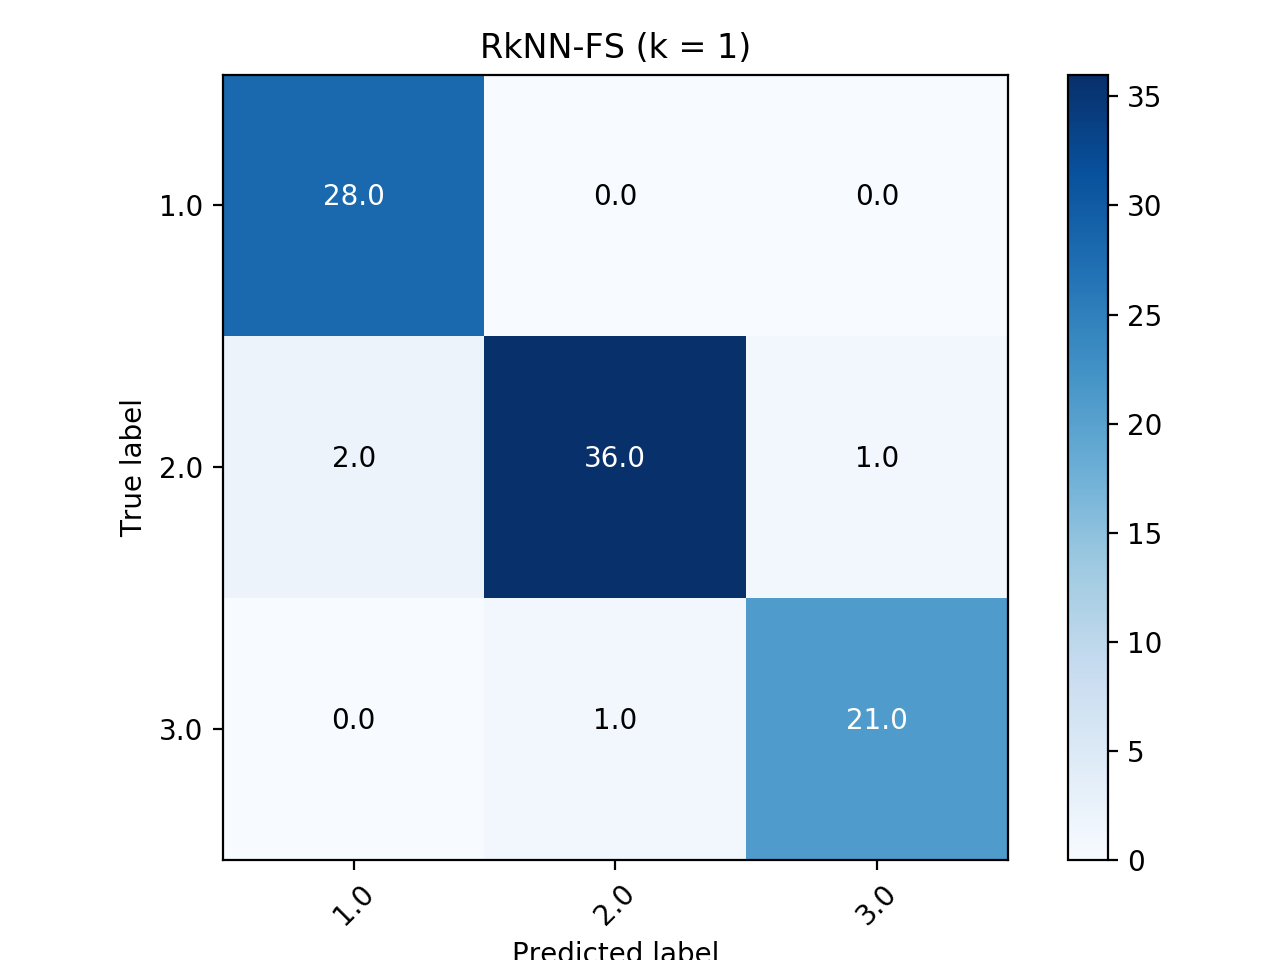
\includegraphics[width=10cm]{r1nn_fs}
		\centering
		\color{blue}
		\caption{Matriu de confusió (algoritme RkNN-FS amb k=1) creada a partir d'una execució sobre les dades d'entrada.}\label{visina8}
	\end{figure}

	\begin{figure}[H]
		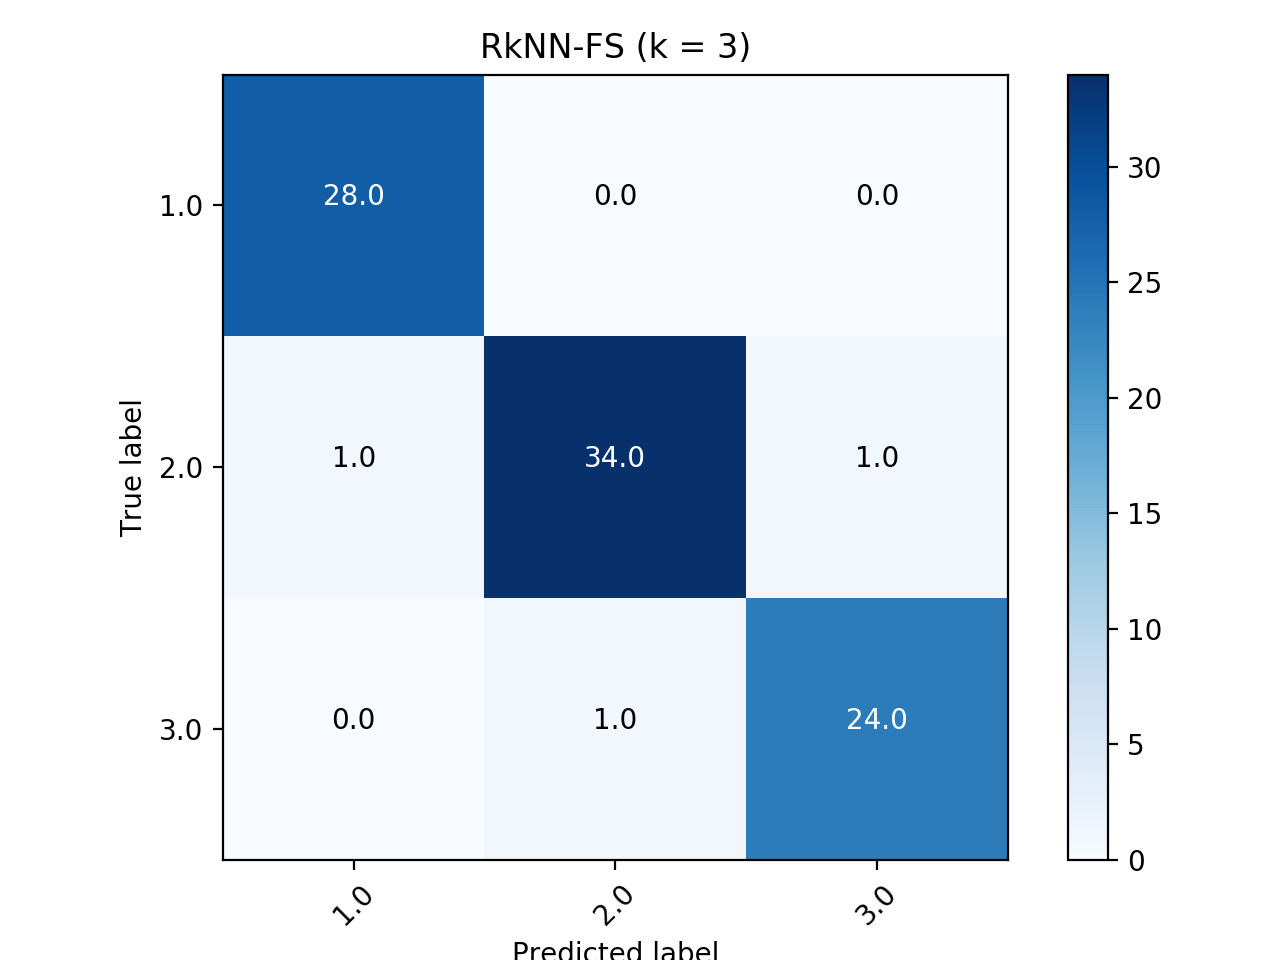
\includegraphics[width=10cm]{r3nn_fs}
		\centering
		\color{blue}
		\caption{Matriu de confusió (algoritme RkNN-FS amb k=3) creada a partir d'una execució sobre les dades d'entrada.}\label{visina8}
	\end{figure}

	També, es pot observar que amb aquest algoritme, el temps dedicat a la selecció de les característiques més importants i a l'entrenament de les dades és molt més gran que en tots els altres algoritmes (de l'ordre d'entre 4500 i 5000 vegades més lent que els kNN, i de 3 i 4 vegades més lent que els RkNN). De totes formes, el temps de predicció, que al final és el temps més rellevant, és el mateix que els kNN ja que el classificador és un kNN entrenat només amb les característiques seleccionades.
}

\end{document}